\documentclass[]{article}

%	Commands
\newcommand{\myTitle}{Sistema de Medición 3D usando Visión Monocular}
\newcommand{\mySubtitle}{}
\newcommand{\myName}{Enrique Mireles Gutierrez}
\newcommand{\myId}{513944}
\newcommand{\myClass}{Robótica Avanzada}
\newcommand{\myProfessor}{Dr. Andrés Hernández Gutiérrez}

%	Doc Properties
\PassOptionsToPackage{portrait, margin=1in}{geometry}
\usepackage{geometry}
\PassOptionsToPackage{parfill}{parskip}
\usepackage{parskip}
\setlength{\parindent}{3em}
\setlength{\parskip}{1em}
\linespread{1.05}

%	Code
\usepackage{minted}

%	Language
\PassOptionsToPackage{spanish}{babel}
\usepackage{babel}
\PassOptionsToPackage{utf8}{inputenc}
\usepackage{inputenc}
\usepackage{gensymb}

%	Math
\usepackage{amsmath}

%	References
\usepackage{url}
\usepackage{apacite}
\bibliographystyle{apacite}

%	Page numbers
\pagestyle{plain}
\pagenumbering{arabic}

%	Pictures
\usepackage{float}
\usepackage{graphicx}
\usepackage[caption = false]{subfig}
\graphicspath{ {./fotos/} }

% Tables
\usepackage{multirow}

\begin{document}

\begin{titlepage}

\centering

\centerline{
\includegraphics{udem}}

\vspace*{2\baselineskip}

{\LARGE \scshape Universidad de Monterrey}\\

\vspace*{2\baselineskip}

{Escuela de Ingeniería y Tecnologías}\\
{\myClass}\\

\vspace*{14\baselineskip}

{\LARGE \myTitle}\\[0.5\baselineskip]
% {\mySubtitle}\\

\vspace*{6\baselineskip}

{Profesor}\\
{\myProfessor}\\

\vspace*{6\baselineskip}

{\myId \qquad \myName}\\



\vspace*{\fill}

{San Pedro Garza García, N.L. a \today}\\

\end{titlepage}

\section{Introducción}

En los últimos años, con los avances en visión computación, el área de reconstrucción 3D ha tenido gran popularidad. Esto ha sido en gran parte por sus diversas aplicaciones que van desde las áreas médicas, la planeación y reconstrucción de edificios, entretenimiento, la robótica, entre muchas otras. Muchos de los algoritmos propuestos buscan lograr una reconstrucción 3D en tiempo real, lo cual presenta grandes dificultades, pero a la vez un gran potencial, sobre todo para los vehículos autónomos.

Es así como existen diversos métodos para realizar una reconstrucción 3D, los cuales se distinguen por la cantidad y el tipo de las cámaras y sensores necesarios para la reconstrucción. Este documento presenta uno de los más sencillos; esto es mediante el uso de una cámara, también conocido como reconstrucción 3D utilizando visión monocular. Tras analizar el modelo matemático detrás de este sistema, se presentan los resultados obtenidos, así como también sus limitantes.

\section{Desarrollo Matemático}

Para poder reconstruir un objeto en 3D utilizando visión monocular necesario comprender el modelo matemático detrás de éste. Una cámara moderna puede ser vista como una cámara obscura. El principio de funcionamiento de esta cámara no es nada nuevo, pues fue descubierta alrededor del año 500 a.C. Esta cámara consiste una caja cerrada con un pequeño orificio a través del cual pasan los rayos de luz y proyectan una imagen invertida en el plano trasero de la caja.

\begin{figure}[H]
	\centering
	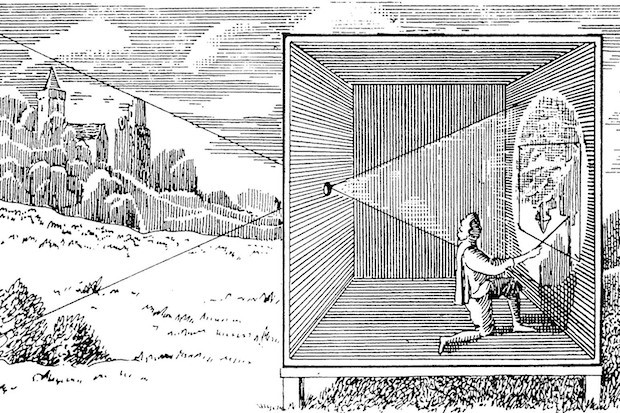
\includegraphics[scale=0.4]{camara-obscura}
	\caption{Representación de una cámara obscura.}
	\label{fig:camara-obscura}
\end{figure}

En la figura \ref{fig:camara-obscura-funcionamiento} se observa como un punto en el espacio $O = [O_x, O_y, O_z]$ es proyectado en el plano de la cámara como $P = [P_x, P_y]$. La distancia focal $f$, es un factor crucial que determina el tamaño de las proyecciones en el material fotosensible.

\begin{figure}[H]
	\centering
	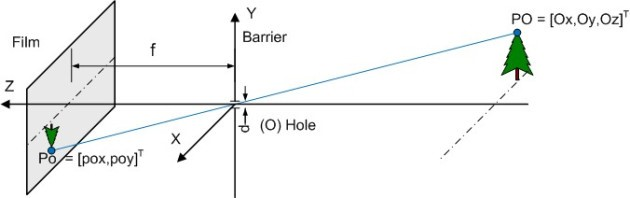
\includegraphics[scale=0.65]{camara-obscura-funcionamiento}
	\caption{Proyección del espacio al plano de la cámara.}
	\label{fig:camara-obscura-funcionamiento}
\end{figure}

Analizando una sola dimensión en la imagen como se muestra en la figura \ref{fig:camara-obscura-triangulos-similares} y utilizando triángulos similares se puede llegar a las formulas que relacionan un punto en el espacio $O$ al plano de la imagen $P$. Resolviendo por las componentes de $O$ se obtiene una manera de pasar de coordenadas en pixeles a coordenadas en el espacio.

\begin{figure}[H]
	\centering
	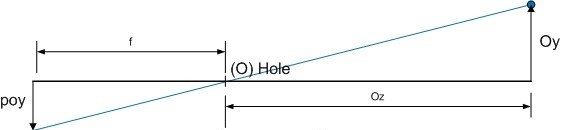
\includegraphics[scale=0.6]{camara-obscura-triangulos-similares}
	\caption{Análisis de triángulos similares en la dirección $-y$.}
	\label{fig:camara-obscura-triangulos-similares}
\end{figure}

\begin{align}
	\label{relacion_2d_3d}
	\frac{P_y}{f} &= \frac{O_y}{O_z} \implies {O_y} = {O_z} * \frac{P_y}{f} \\
	\frac{P_x}{f} &= \frac{O_x}{O_z} \implies {O_x} = {O_z} * \frac{P_x}{f}
\end{align}

A diferencia de una cámara obscura, las cámaras de hoy en día utilizan un lente convexo para concentrar la mayor cantidad de luz en el material foto sensible o sensor fotográfico al fondo de la cámara. A pesar de ello, analizando triángulos similares en las direcciones $-x$ y $-y$ se llegan a las mismas formulas presentadas anteriormente.

\begin{figure}[H]
	\centering
	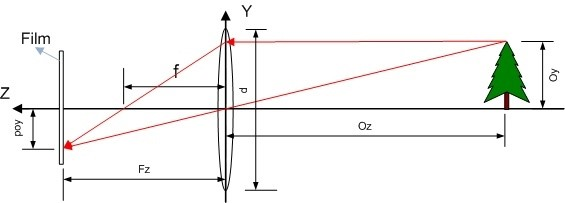
\includegraphics[scale=0.6]{camara-lente}
	\caption{Análisis de una cámara con lente.}
	\label{fig:camara-lente}
\end{figure}

Al utilizar un lente convexo se introduce el problema de las distorsiones radiales y tangenciales. Estas distorsiones se deben a que la fabricación de las cámaras no es perfecta. Al intentar reconstruir escenas 3D con una cámara con distorsiones el problema se vuelve complicado. Para corregir esto es necesario realizar una calibración, la cual permite obtener los parámetros que describen esas distorsiones también conocidos como parámetros intrínsecos y extrínsecos de la cámara. Utilizando estos parámetros es posible corregir una imagen para eliminar las distorsiones.

Una vez que se obtiene una imagen corregida es posible realizar la reconstrucción 3D. La clave de ello con una cámara monocular es conocer la distancia $O_z$ a la que se encuentra el objeto. Teniendo esta información y la distancia focal de la cámara (obtenida de la calibración) se pueden obtener las coordenadas reales del objeto en el espacio. Esto se hace mediante las formulas en \ref{relacion_2d_3d}.

Para conocer la distancia $O_z$ existen diversos métodos, muchos de los cuales se basan en los principios de la cámara estéreo y sensores externos. Sin embargo, estos sistemas están fuera del alcance de este proyecto. Por eso la distancia $O_z$ es medida de manera manual e introducida en el programa como será mostrado en la siguiente sección. Conociendo $O_z$, la distancia focal $f$ y asumiendo que los puntos a medir se encuentran en el mismo plano, es posible calcular sus equivalentes en el espacio. Tomando dos puntos de la imagen $P_1 = [P_{1x}, P_{1y}]$ y $P_2 = [P_{2x}, P_{2y}]$ se transforman al espacio de la siguiente manera:

\begin{align}
	O_1 &= [O_{1x}, O_{1y}] = [O_z * P_{1x} / f, O_z * P_{1y} / f]\\
	O_2 &= [O_{2x}, O_{2y}] = [O_z * P_{2x} / f, O_z * P_{2y} / f]
\end{align}

Una vez teniendo $O_1$ y $O_2$ se puede calcular la distancia Euclidiana entre ellos. Dado que ambos puntos se encuentran en el mismo plano la componente en $Z$ de la formula se hace $0$.

\begin{align}
	d &= \sqrt{(O_{1x} - O_{2x})^2 + (O_{1y} - O_{2y})^2 + (O_{z} - O_{z})^2}\\
	d &= \sqrt{(O_{1x} - O_{2x})^2 + (O_{1y} - O_{2y})^2} 
\end{align}

\section{Uso del Programa}

Para demostrar el método propuesto se programó un sistema de reconstrucción 3D en Python 3 utilizando OpenCV. El programa es ejecutado desde la línea de comandos utilizando el siguiente formato:

\begin{minted}{bash}
	python3 3d.py config cam distance
\end{minted}

\noindent Además, es posible obtener ayuda sobre cómo introducir los comandos y qué significa cada uno de ellos con la siguiente instrucción:

\begin{minted}{bash}
	python3 3d.py -h
\end{minted}

\begin{figure}[H]
	\centering
	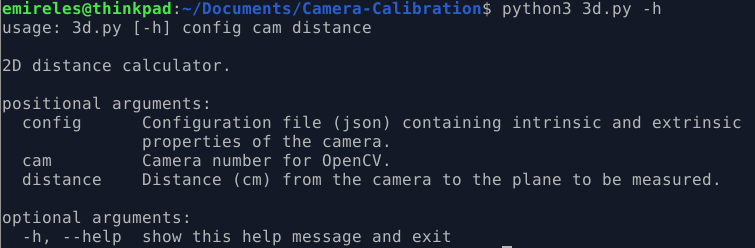
\includegraphics[scale=0.7]{programa-help}
	\caption{Salida del comando de ayuda del programa.}
	\label{fig:programa-help}
\end{figure}

El archivo de configuración necesario para la ejecución del programa es del tipo .json y contiene información sobre los parámetros intrínsecos y extrínsecos de la cámara. El formato del archivo de configuración es el siguiente:

\begin{minted}{json}
{
	"focal_length": 806.818858268,
	"width": 640,
	"height": 480,
	"cx": 320,
	"cy": 240
}
\end{minted}

Tras realizar la medición manual desde la cámara hasta el plano en el que se encuentran los objetos e introducirla en los parámetros del programa se puede proceder a realizar la medición. El programa muestra a la derecha una imagen de 50x50 pixeles escalada en la posición actual del cursor. Esto es para permitirle al usuario seleccionar con mayor precisión el píxel deseado.

\begin{figure}[H]
	\centering
	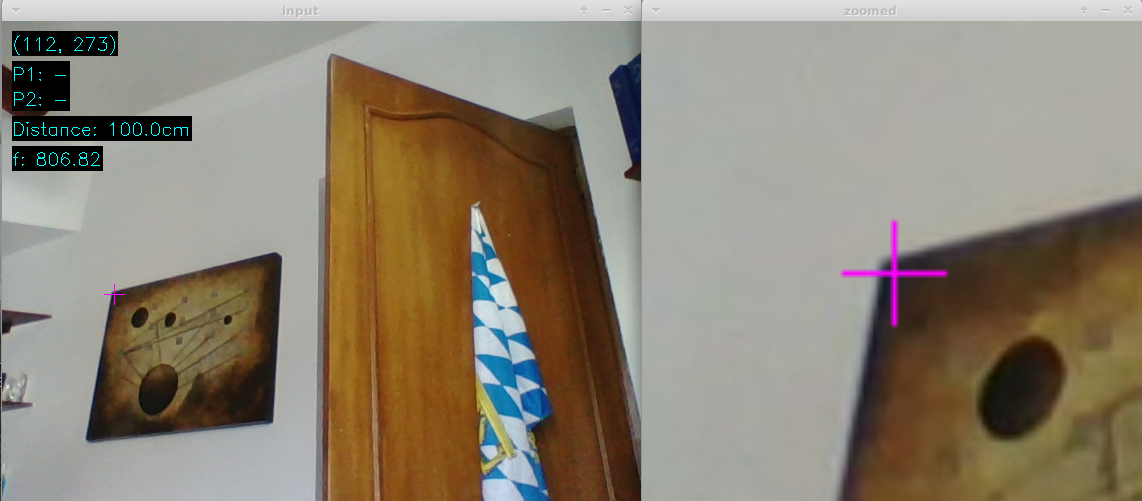
\includegraphics[scale=0.5]{programa-gui}
	\caption{Interfaz de usuario del programa.}
	\label{fig:programa-gui}
\end{figure}

El procedimiento consiste en seleccionar dos puntos y tras ello la distancia en centímetros será presentada al usuario. En caso de querer realizar otra medición, simplemente se seleccionan otros dos puntos y el programa automáticamente realizará una nueva medición.

\begin{figure}[H]
	\centering
	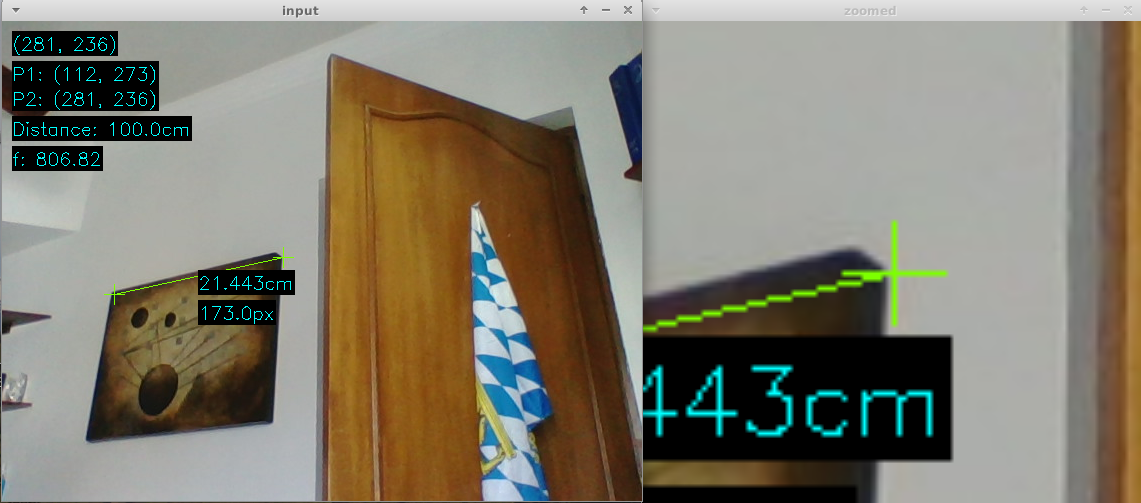
\includegraphics[scale=0.5]{programa-gui-medicion}
	\caption{Resultado de la medición.}
	\label{fig:programa-gui-medicion}
\end{figure}

\section{Resultados Experimentales}

Para evaluar el funcionamiento del sistema se optó por realizar mediciones de cinco objetos distintos a dos distancias diferentes. La primera prueba se realizó a 662 mm y la segunda a 895 mm. Las dimensiones reales de los objetos fueron medidas con un vernier con precisión de $\pm$ 0.1mm. Además, todas las mediciones son presentadas en milímetros.

\begin{table}[H]
	\centering
	\begin{tabular}{|c|c|c|c|c|c|c|}
		\hline
		\multirow{2}{*}{\textbf{Objeto}} & \multirow{2}{*}{\textbf{Real}} & \multicolumn{2}{c|}{\textbf{Altura 1 (662 mm)}} & \multirow{2}{*}{\textbf{Promedio}} & \multirow{2}{*}{\textbf{Error Abs}} & \multirow{2}{*}{\textbf{Error \%}} \\ \cline{3-4}
		 &  & \textbf{Muestra 1} & \textbf{Muestra 2} &  &  &  \\ \hline
		Vernier & 30,00 & 30,90 & 29,64 & 30,27 & -0,27 & -0,9\% \\ \hline
		Batería de 9V & 44,79 & 43,79 & 44,98 & 44,39 & 0,41 & 0,9\% \\ \hline
		Caja de Mentas & 65,00 & 65,69 & 66,07 & 65,88 & -0,88 & -1,4\% \\ \hline
		Tarjeta & 85,50 & 86,00 & 83,69 & 84,85 & 0,66 & 0,8\% \\ \hline
		Pluma & 168,00 & 167,19 & 170,27 & 168,73 & -0,73 & -0,4\% \\ \hline
	\end{tabular}
	\label{table:resultados-1}
	\caption{Análisis de resultados a z = 662 mm.}
\end{table}

\begin{figure}[h]
	\centering
	\subfloat[Vernier]{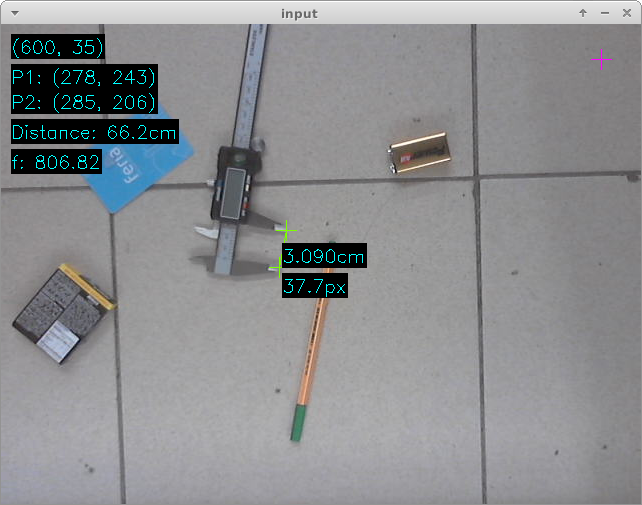
\includegraphics[width = 2.2in]{P1-VERNIER}} 
	\subfloat[Bateria]{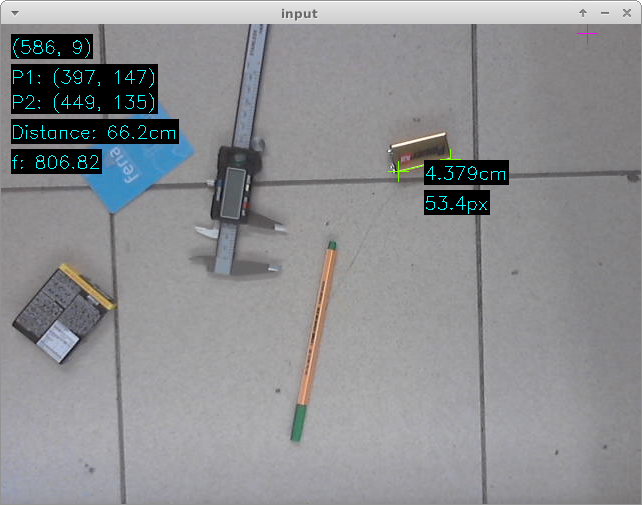
\includegraphics[width = 2.2in]{P1-BAT}}
	\subfloat[Caja de Mentas]{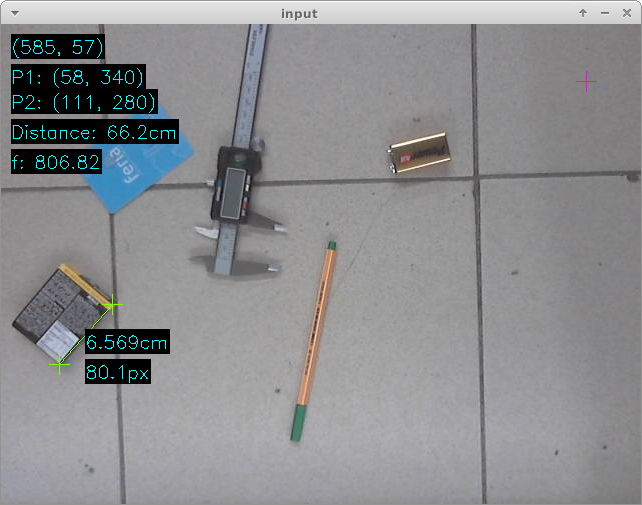
\includegraphics[width = 2.2in]{P1-HALLS}}\\
	\subfloat[Pluma]{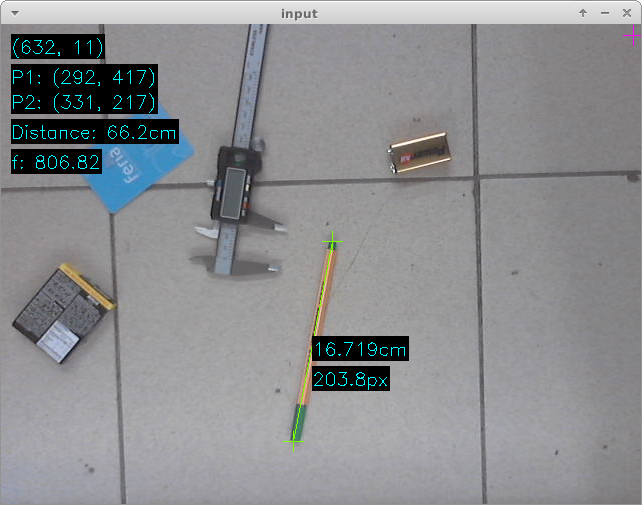
\includegraphics[width = 2.2in]{P1-STABILO}}
	\subfloat[Tarjeta]{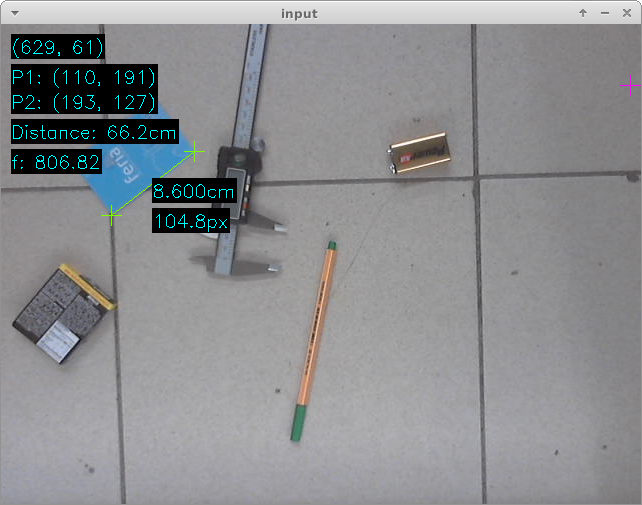
\includegraphics[width = 2.2in]{P1-FERIA}}
	\caption{Resultados a z = 662 mm.}
	\label{fig:resultados-1}
\end{figure}

\begin{table}[H]
	\centering
	\begin{tabular}{|c|c|c|c|c|c|c|}
		\hline
		\multirow{2}{*}{\textbf{Objeto}} & \multirow{2}{*}{\textbf{Real}} & \multicolumn{2}{c|}{\textbf{Altura 2 (895 mm)}} & \multirow{2}{*}{\textbf{Promedio}} & \multirow{2}{*}{\textbf{Error Abs}} & \multirow{2}{*}{\textbf{Error \%}} \\ \cline{3-4}
		 &  & \textbf{Muestra 1} & \textbf{Muestra 2} &  &  &  \\ \hline
		Vernier & 30,00 & 30,54 & 30,14 & 30,34 & -0,34 & -1,1\% \\ \hline
		Batería de 9V & 44,79 & 42,69 & 46,29 & 44,49 & 0,30 & 0,7\% \\ \hline
		Caja de Mentas & 65,00 & 67,75 & 67,05 & 67,40 & -2,40 & -3,7\% \\ \hline
		Tarjeta & 85,50 & 86,82 & 83,96 & 85,39 & 0,11 & 0,1\% \\ \hline
		Pluma & 168,00 & 170,77 & 169,12 & 169,95 & -1,94 & -1,2\% \\ \hline
		\end{tabular}
	\label{table:resultados-2}
	\caption{Análisis de resultados a z = 895 mm.}
\end{table}


\begin{figure}[H]
	\centering
	\subfloat[Vernier]{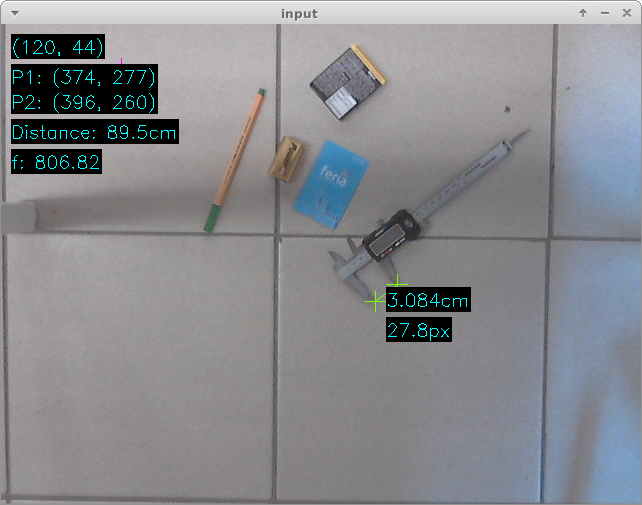
\includegraphics[width = 2.2in]{P2-VERNIER}} 
	\subfloat[Bateria]{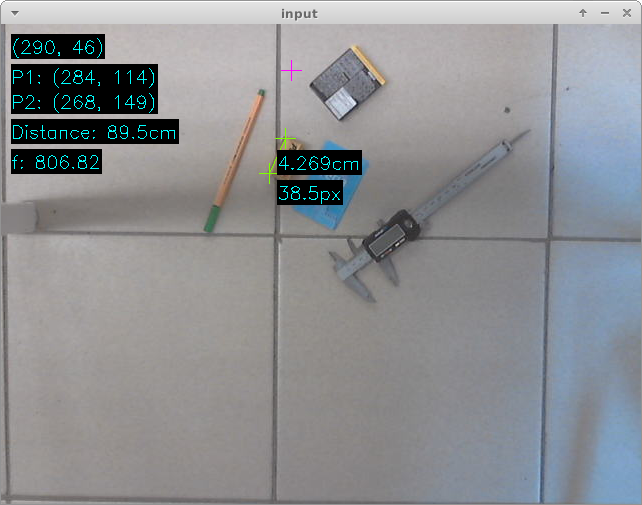
\includegraphics[width = 2.2in]{P2-BAT}}
	\subfloat[Caja de Mentas]{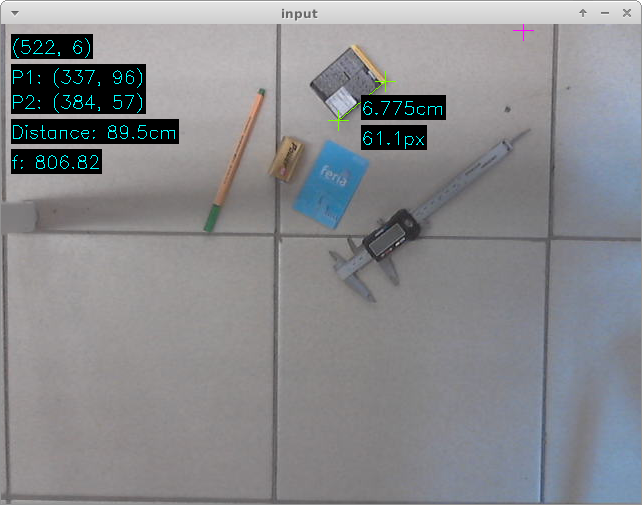
\includegraphics[width = 2.2in]{P2-HALLS}}\\
	\subfloat[Pluma]{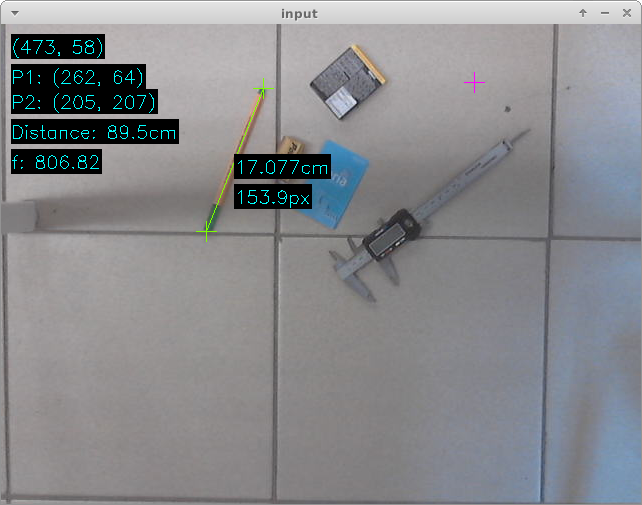
\includegraphics[width = 2.2in]{P2-STABILO}}
	\subfloat[Tarjeta]{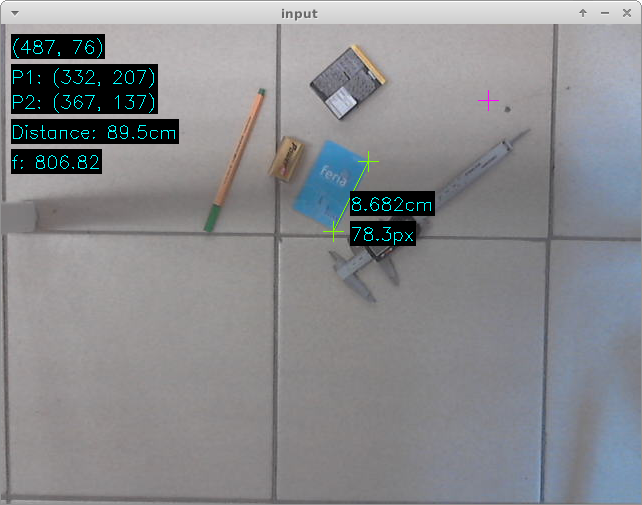
\includegraphics[width = 2.2in]{P2-FERIA}}
	\caption{Resultados a z = 895 mm.}
	\label{fig:resultados-2}
\end{figure}

\section{Discusión de Resultados Experimentales}

Analizando los resultados se observa que el error absoluto en la mayoría de las mediciones fue inferior a 1 mm.  Sucedieron dos casos a la distancia mayor en los que el error absoluto fue mayor a 1 mm, específicamente fue de 2.4 mm y 1.94 mm. En general, el error porcentual estuvo cerca del 1\%.

Sin duda, la resolución de la cámara tiene un papel muy importante. A una mayor resolución hay más pixeles sobre cuales escoger los puntos $P_1$ y $P_2$. Esta prueba se realizó a 640x480 pixeles. En casó de utilizar una resolución mayor se pueden obtener mejores resultados. Además, la exactitud con la se escogen los puntos depende del usuario, lo cual introduce un error a la medición. No siempre el usuario hará clic sobre el mismo píxel dos veces seguidas.

Otro error que se presenta en la medición es que no todos los objetos se encuentran sobre el mismo plano -z. La altura de algunos objetos difiere, lo cual hace que la componente -z del calculo presentado anteriormente no sea 0 y tenga un efecto, aunque no tan significativo como el factor humano en la medición.


\section{Conclusiones}

El sistema presentado es capaz de medir las dimensiones de objetos con una alta precisión. Además, el costo del sistema es bastante barato, ya que solamente utiliza una cámara web de aproximadamente \$250 MXN. La combinación de estas dos características brinda un sistema atractivo y sencillo para medir dimensiones en un plano. A pesar de ello existen muchas áreas de oportunidad para el 
sistema.

Una limitante del sistema es que hay que introducir manualmente la distancia a la que encuentran los objetos. Esto puede ser solucionado agregando algún sensor de distancia o incluso un láser y analizando cómo es que el punto se desplaza en la imagen determinar la distancia de la cámara al plano. Otro problema surge cuando hay objetos que no están sobre el mismo plano. En caso de querer medir objetos a diferentes distancias en Z es necesario utilizar otras técnicas. Una posible solución podrá ser un utilizar un láser de línea y analizando la distorsión de la línea se puede calcular la altura de los objetos.

Tomando todo esto en cuenta, el solucionar las limitantes del sistema propuesto introduce una mayor complejidad. Lo atractivo del sistema propuesto es su simpleza con la que puede ser implementado y la calidad de los resultados que se pueden obtener.

\nocite{a}
\nocite{b}
\nocite{c}
\nocite{d}
\nocite{e}
\nocite{f}

{\raggedright\bibliography{referencias}}

\begin{center}
	\vspace*{\fill}
	Doy mi palabra de que he realizado esta actividad con honestidad académica.
\end{center}

\end{document}